\documentclass{ltjsarticle}

\usepackage{amsmath}
\usepackage{amssymb}
\usepackage{amsthm}
\usepackage{ mathrsfs }
\usepackage{enumerate}
\usepackage{bbm}
\usepackage{lipsum}
\usepackage{fancyhdr}
\usepackage{tikz-cd} 
\usetikzlibrary{graphs}
\usepackage{luatexja-ruby} 
\usepackage{graphicx} 
\graphicspath{ {./../../images/} }

\newtheorem{theorem}{定理}[section] 
\newtheorem{proposition}{Proposition}[section] 
\newtheorem{definition}{定義}[section] 
\newtheorem{problem}{問題}
\newtheorem{postulate}{公準}[section] 
\newtheorem{lemma}{Lemma}[section] 
\newtheorem{notation}{Notation}[section] 
\newtheorem{remark}{注釈}[section] 
\newtheorem{corollary}{系}[section] 
\newtheorem{terminology}{Terminology}[section] 
\newtheorem{example}{例}[section] 
\newtheorem{step}{手順} 
\newtheorem{solution}{解答}[section] 
\newtheorem{fact}{事実}[section] 

\DeclareMathOperator{\diam}{diam}
\DeclareMathOperator{\Gal}{Gal}
\DeclareMathOperator{\rank}{rank}
\DeclareMathOperator{\Hom}{Hom}
\DeclareMathOperator{\Dom}{Dom}
\DeclareMathOperator{\Ann}{Ann}
\DeclareMathOperator{\grad}{grad}
\DeclareMathOperator{\Span}{Span}
\DeclareMathOperator{\interior}{int}
\DeclareMathOperator{\ind}{ind}
\DeclareMathOperator{\supp}{supp}
\DeclareMathOperator{\ob}{ob}
\DeclareMathOperator{\Spec}{Spec}
\DeclareMathOperator{\MaxSpec}{MaxSpec}
\DeclareMathOperator{\PreSh}{PreSh}
\DeclareMathOperator{\Sh}{Sh}
\DeclareMathOperator{\Fun}{Fun}
\DeclareMathOperator{\Ext}{Ext}
\DeclareMathOperator{\Aut}{Aut}
\DeclareMathOperator{\Ker}{Ker}
\DeclareMathOperator{\Image}{Im}
\DeclareMathOperator{\Coker}{Coker}
\DeclareMathOperator{\id}{id}
\DeclareMathOperator{\Mod}{Mod}
\DeclareMathOperator{\QCoh}{QCoh}
\DeclareMathOperator{\Coh}{Coh}
%\newcommand*{\name}[\num_arguments][default values]{{\color{#1}\Large #2}}
\newcommand*{\Z}{\mathbb{Z}}
\newcommand*{\Q}{\mathbb{Q}}
\newcommand*{\R}{\mathbb{R}}
\newcommand*{\multivar}[2]{{#1_1,\cdots,#1_{#2}}}
\newcommand*{\localization}[2]{#1_{\mathfrak{#2}}}
\newcommand*{\ringedspacemorph}[1]{(#1,#1^{\#})}
\newcommand*{\sheaf}[2]{(#1,{\mathcal{#2}}_{#1})}
\newcommand{\fib}[1]{%
  \mathbin{\mathop{\times}\limits_{#1}}%
}
\newcommand{\tens}[1]{%
  \mathbin{\mathop{\otimes}\displaylimits_{#1}}%
}
\title{授業ノート}
\author{ボン補習校高校数学}
\date{５月１６日}

\begin{document}

\maketitle

\section{問題の答え}
\par\textbf{微分}
\par\textbf{問題：}次の関数の微分を計算せよ。
\begin{equation*}
3x^2+x+1,x^3+3x^2+3x+1,3e^x+5x
\end{equation*}
\par\textbf{解答：}
$x^n$の微分は$nx^{n-1}$だったことを思い出しましょう。よって順番に最初は
\begin{equation*}
(3x^2+x+1)' = (3x^2)'+(x)'+(1)' = 3(x^2)+(x)'+(1)' = 3\cdot 2x+1+0 = 6x+1
\end{equation*}
二番目は
\begin{equation*}
(x^3+3x^2+3x+1)' = (x^3)'+(3x^2)'+(3x)'+(1)' = (x^3)'+3(x^2)'+3(x)'+(1)'  = 3x^2+3\cdot 2x+3x+0 = 3x^2+6x+3x
\end{equation*}
最後は
\begin{equation*}
(3e^x+5x)' = (3e^x)'+(5x)'= 3(e^x)'+5(x)' = 3e^x +5
\end{equation*}
\textbf{問題：}$e^x$の$x=0$での接線を求めて、元のグラフとの差が
\begin{equation*}
{\frac {x^2} {2!}}+{\frac {x^3} {3!}}+\cdots
\end{equation*}
になることを確認しよう。
\par \textbf{チャレンジ課題：変数変換}
\par 二つの微分可能な関数$f,u$について$(f\circ u)(x) = f(u(x))$とします。例えば$f(x) = x^2, u=x+1$なら$(f\circ u)(x) = (x+1)^2$となります。ここで$f\circ u$の微分を考えてみましょう。
\begin{equation*}
\lim_{h\to 0}{\frac {f(u(x+h))-f(u(x))} {h}} \stackrel{1={\frac {u(x+h)-u(x)} {u(x+h) -u(x)}}\text{を掛けて}}{=} \lim_{h\to 0}{\frac {u(x+h)-u(x)} {h}}\cdot\lim_{h\to 0}{\frac {f(u(x+h))-f(u(x))} {u(x+h)-u(x)}}
\end{equation*}
ここで極限の定義を思い出しましょう。
\begin{equation*}
\lim_{x\to a}g(x)= \alpha
\end{equation*}
になると言うのはどんな数列$(a_n)_{n=1,2,\cdots}$でももし
\begin{equation*}
\lim_{n\to\infty}a_n = a
\end{equation*}
となるなら、
\begin{equation*}
\lim_{n\to \infty}g(a_n) = \alpha
\end{equation*}
となることでした。ここで$u(x)$は連続なので$\lim_{h\to 0}u(x+h)$は$h$をそのまま代入して
\begin{equation*}
\lim_{h\to0}u(x+h) = u(x+0) =  u(x)
\end{equation*}
となります。なので
\begin{equation*}
\lim_{h\to 0}(u(x+h)-u(x)) =   u(x+0) - u(x) = u(x)-u(x) = 0
\end{equation*}
ここで$a_n = u\left(x+{\frac 1 n}\right)-u(x)$とおくと
\begin{equation*}
\lim_{n\to\infty}a_n = \lim_{n\to\infty}u\left(x+{\frac 1 n}\right)-u(x) = \lim_{h\to 0 }u(x+h)-u(x) = 0
\end{equation*}
また
\begin{equation*}
u\left(x+{\frac 1 n}\right) = u\left(x+{\frac 1 n}\right) - u(x)+u(x) = a_n+u(x)
\end{equation*}
これを使って
\begin{align*}
 \lim_{h\to 0}{\frac {f(u(x+h))-f(u(x))} {u(x+h)-u(x)}} &=  \lim_{n\to \infty}{\frac {f\left(u\left(x+{\frac 1 n}\right)\right)-f(u(x)} {a_n}},\\
 &=\lim_{n\to \infty}{\frac {f(u(x)+a_n)-f(u(x))} {a_n}},\\
 & = \lim_{h\to0}{\frac {f(u(x)+h)-f(u(x))} {h}}
 & = f'(u(x)).
\end{align*}
となります。$\lim_{h\to 0}{\frac {u(x+h)-u(x)} {h}} = u'(x)$なので掛け算すると
\begin{align*}
(f\circ u)'(x)&= \lim_{h\to 0}{\frac {f(u(x+h))-f(u(x))} {h}},\\
& = \lim_{h\to 0}{\frac {u(x+h)-u(x)} {u(x+h)-u(x)}}\cdot{\frac {f(u(x+h))-f(u(x))} {h}},\\
& = \lim_{h\to 0}{\frac {u(x+h)-u(x)} {h}}\cdot{\frac {f(u(x+h))-f(u(x))} {u(x+h)-u(x)}},\\
& = \left(\lim_{h\to 0}{\frac {u(x+h)-u(x)} {h}}\right)\left(\lim_{h\to0}{\frac {f(u(x+h))-f(u(x))} {u(x+h)-u(x)}}\right),\\
&= u'(x)f'(u(x)).
\end{align*}
となります。
\par\textbf{例：}$(x+1)^2$の微分を$f(x) = x^2,u(x) = x+1$とすると$f\circ u(x) = (x+1)^2$なるまた$f'(x) = 2x,u'(x) = 1$よって
\begin{equation*}
((x+1)^2)' = (f\circ u)'(x) = 1\cdot 2(x+1)
\end{equation*}
\par\textbf{チャレンジ問題：}次の関数の微分をしてみよう。
\begin{equation*}
(x+1)^3,(2x+1)^2(x^2+2)^4
\end{equation*}
\textbf{解答}\\
$f(x) = x^3,u(x)=(x+1)$とおくと $f'(x) = 3x^2,u'(x) = 1$なので、
\begin{equation*}
((x+1)^3)' = (f\circ u)'(x) = u'(x)\cdot f'(u(x)) = 1 \cdot 3(x+1)^2 = 3(x+1)^2
\end{equation*}
$f(x) = x^2,u(x)=(2+1)$とおくと $f'(x) = 2x,u'(x) = 2$なので、
\begin{equation*}
((2x+1)^2)' = (f\circ u)'(x) = u'(x)\cdot f'(u(x)) = 2 \cdot 2(2x+1) = 4(2x+1)
\end{equation*}
$f(x) = x^4,u(x)=(x^2+2)$とおくと $f'(x) = 4x^3,u'(x) = 2x$なので、
\begin{equation*}
((x^2+2)^4)' = (f\circ u)'(x) = u'(x)\cdot f'(u(x)) = 2x \cdot 4((x^2+2))^3= 8x(x^2+1)^3
\end{equation*}
\par\textbf{グラフ理論：オイラーグラフ}\\
\textbf{問題：}次のグラフを一筆で書くことを考える。
\begin{center}
\begin{figure}[h]
	\centering
    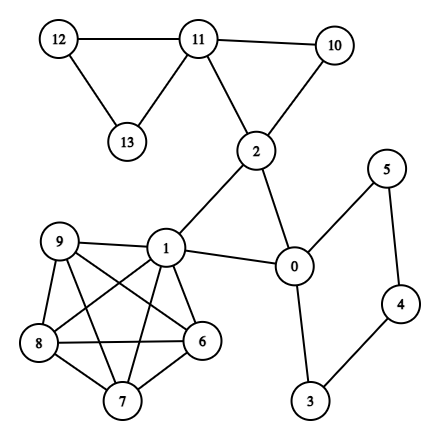
\includegraphics[scale=0.25]{euler_graph_big}
    \label{fig:Euler_1}
\end{figure}
\end{center}
\begin{center}
最初のグラフからまんなかの$0-1-2$のサイクルを取り除いたグラフ
\begin{figure}[h]
	\centering
    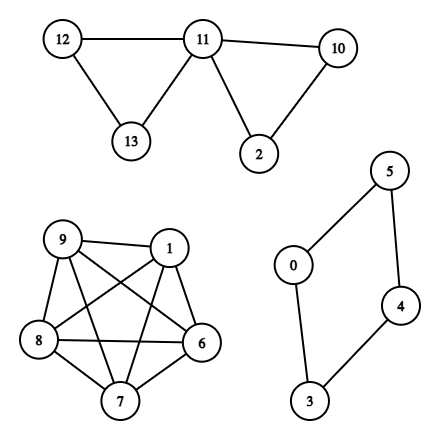
\includegraphics[scale=0.25]{euler_graph_disconnected}
    \label{fig:Euler_1}
\end{figure}
\end{center}
$\:$\\\\\\\\\\\\\ 三つのグラフに分かれました。それぞれ一筆書きできますか？これをつかって元のグラフを一筆書きすることを考えてみましょう。
\par\textbf{チャレンジ問題：}もし元のグラフが一筆で書けるなら、そこからサイクルを取り除いたグラフは一筆書きできるいくつかのグラフに分かれます。これはなぜでしょうか。（サイクルの辺を取り除いた時繋がれていた頂点はそれぞれいくつ次数が減ったかな？）
\par\textbf{解答}
一筆書きできるグラフの頂点の次数は全て偶数であることを先週のクラスでは見ました。サイクルを見てみましょう
\begin{figure}[h]
	\centering
    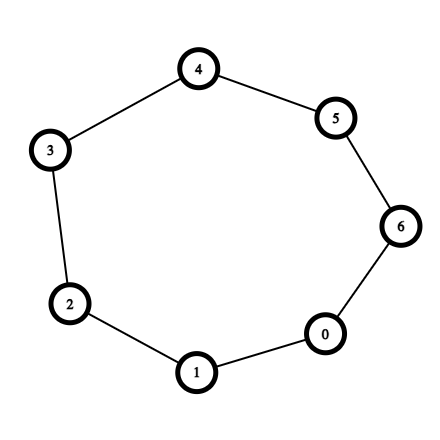
\includegraphics[scale=0.25]{cycle_example}
    \label{fig:cycle_1}
\end{figure}
\end{center}
上の図から分かるようにサイクルのそれぞれの頂点の次数は$2$です。よってグラフの中のサイクルを消すと、サイクルに含まれている頂点の次数は$2$へって、含まれていない頂点の次数はそのままになります。つまり、全ての頂点の次数は偶数のままとなるのです。
\par\textbf{整数論：合同式}

$n$を整数とする時、二つの整数$a,b$が$n$を法として合同とは$b-a$が$n$で割れる時、言い換えて$a,b$の$n$で割った時の余りが同じことを言います。これを
\begin{equation*}
a\equiv b\mod{n}
\end{equation*}
と書きます。これを使うと全ての整数を$n$で割った余りで分類することができます。
\par\textbf{問題：}$n=2,3,7,11$の時それぞれ可能な余りはいくつですか。例えば$n=5$のとき可能な余りは$0,1,2,3,4$です。
\par\textbf{問題：}次の二つを証明してみましょう。もし$a\equiv b\mod{n},c\equiv d\mod{n}$ならば
\begin{enumerate}
\item $a+c\equiv b+d\mod{n}$
\item $ac \equiv bd\mod{n}$
\end{enumerate}

\par\textbf{ステップ１：}示したいのは
\begin{equation*}
(b+d)-(c+a)
\end{equation*}
が$n$で割れること。私たちが知っているのは
\begin{equation*}
(b-a),(d-c)
\end{equation*}
が$n$で割れること（二つは$n$の約数）。これを使って$(c+d)-(a+b)$を$n$の約数の和にできないだろうか。
\par\textbf{解答}\\
\begin{equation*}
(b+d)-(c+a) = (b-a)+(d-c)
\end{equation*}
これは$n$の約数の和。
\par\textbf{ステップ２：}最初と同じように$bd-ac$が$n$で割れることを知りたい。
$bc-bc = 0$なので
\begin{equation*}
bd-ac = bd-ac+0 = bd-ac -bc+bc
\end{equation*}
最後の形をうまく変形して$n$の倍数の和にしよう。
\par\textbf{解答}\\
\begin{equation*}
bd-ac = bd-bc+bc-ac = b(d-c)+c(b-a)
\end{equation*}
これも$n$の約数の和。
\par\textbf{問題：}$2^{100}$と$3^{100}$の一の位の数を調べてみよう。ここで、

\begin{align*}
2^1 &\equiv 2 \mod{10},2^2 \equiv 4 \mod{10},2^3 \equiv 8 \mod{10}\\
2^4 &\equiv 16 \equiv 6 \mod{10},2^5\equiv 32 \equiv 2 \mod{10},
\end{align*}
になることに注意しよう。指数法則をつかうと$(2^a)^b = 2^{ab}$となります。最初の問題で見たように、余りの式では掛け算が使えます。なので指数法則はあまりの式でも使えます。例えば上の式で$2^5\equiv 2\mod{10}$なので、
\begin{equation*}
2^{10} \equiv 2^{5\times 2} \equiv (2^5)^2 \equiv 2^2 \equiv 4 \mod{10}
\end{equation*}
つまり$2^{10}$の一の位は$4$。これを使って$2^{100},3^{100}$の一の位の数を調べてみよう。

\par\textbf{解答}\\
\begin{equation*}
2^{10} \equiv 1024 \equiv 4\mod{10}
\end{equation*}
なので
\begin{align*}
2^{100}& \equiv (2^{10})^{10}\equiv (1024)^{10)} \equiv 4^{10},\\
&\equiv (2^2)^{10} \equiv (2)^{20}\equiv (2^{10})^2 \equiv (4)^2  \equiv 6\mod{10}.
\end{align*}
同じように
\begin{equation*}
3^{4} \equiv 81 \equiv 1\mod{10}
\end{equation*}
なので
\begin{equation*}
3^{100} \equiv (3^{4})^{25} \equiv (81)^{25} \equiv (1)^{25)} \equiv 1\mod{10}.
\end{equation*}
\par\textbf{図形：三角形の外心と内心}\\
\textbf{問題：}$OD,OE$はそれぞれ辺$AB,BC$を垂直に半分にする線。ここで$OA=OB=OC$となることを確かめよう。また$F$がちょうど辺$CA$の真ん中の時$OF$が$CA$に垂直になること示そう。（ヒント：この問題は$\triangle OAB,\triangle OBC$がそれぞれ二等辺三角形になることを聞いています。そのことを証明するためにどのような合同な三角形を見つければ良いでしょうか。）
\begin{center}
\begin{figure}[h]
	\centering
    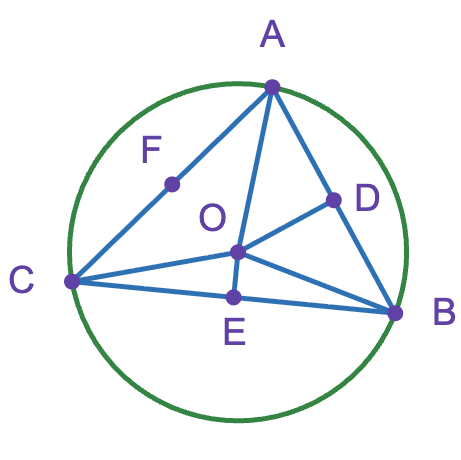
\includegraphics[scale=0.25]{outer_center}
    \label{fig:Euler_1}
\end{figure}
\end{center}
\textbf{解答}\\
三角形$OEC,OEB$は
\begin{equation*}
OE = OE, CE \stackrel{\text{$E$は線$BC$の真ん中}}{=} EB,\angle OEC = \angle OEB = 90^\circ
\end{equation*}
なので合同、よって$OC=OB$となる。同じように
\begin{equation*}
OD = OD, AD \stackrel{\text{$D$は線$AB$の真ん中}}{=} DB,\angle ODA = \angle ODB = 90^\circ
\end{equation*}
なので$OA=OB$。$OF,CA$が垂直なのは二つの三角形$\triangle OFA,\triangle OFC$が
\begin{equation*}
AF = FC, OF = OF, OA = OC
\end{equation*}
となるので合同。よって
\begin{equation*}
\angle OFC = \angle OFA, \angle OFC+\angle OFA = 180^\circ
\end{equation*}
となるので
\begin{equation*}
\angle OFC+\angle OFA = 2\angle OFC = 180^\circ
\end{equation*}
より$\angle OFC = 90^\circ$.
\par \textbf{問題：}$OA,OB$は角$A,B$をそれぞれ半分にする線です。ここで$OI,OG$をそれぞれ$AB,BC$に垂直な線とすると$OI=OG$となることを示そう。また$CA$上の点$H$を$OH$が$CA$に垂直になるように引くと、$OH=OI=OG$になることと$OC$が角$C$を半分にすることも示そう。（ヒント：外心の時と同じように合同な三角形を見つけてみよう。最後の部分はピタゴラスの定理を使うと簡単になります。）
\begin{center}
\begin{figure}[h]
	\centering
    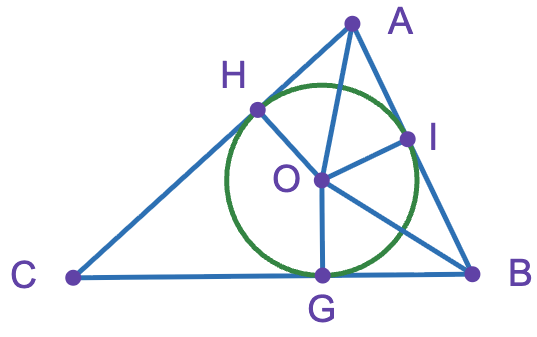
\includegraphics[scale=0.25]{inner_center}
    \label{fig:Euler_1}
\end{figure}
\end{center}
\textbf{解答}\\
\begin{equation*}
\angle AIO = \angle AHO = 90^\circ, \angle HAO \stackrel{\text{$OA$は角$HAI$を半分にする}}{=} \angle OAI ,AO = AO
\end{equation*}
なので$\triangle HAO,\triangle OAI$は合同よって
\begin{equation*}
OH = OI
\end{equation*}
同じように
\begin{equation*}
\angle BIO = \angle BGO = 90^\circ, \angle IBO \stackrel{\text{$OA$は角$HAI$を半分にする}}{=} \angle OBG ,BO = BO
\end{equation*}
なので$\triangle IBO,\triangle OBG$は合同よって
\begin{equation*}
OI = OG
\end{equation*}
ここで$\angle OHC=\angle OGC = 90^\circ$なのでピタゴラスの定理を使うと
\begin{equation*}
OC^2=OH^2+HC^2, OC^2 = OG^2+GC^2
\end{equation*}
つまり
\begin{equation*}
OH^2+HC^2= OG^2+GC^2
\end{equation*}
となります$OH=OG$となるので
\begin{equation*}
OH^2+HC^2 = OH^2+GC^2
\end{equation*}
よって$HC = GC$。二つの三角形$\triangle OHC,\triangle OGC $は合同になるので
\begin{equation*}
\angle OCH = \angle OCG
\end{equation*}
つまり$OC$は角$C$を半分にする。
\section{やってきたことのおさらい}

円周率とは直径と円周の長さの比であることを思い出しましょう。昔に人は次のように円周率の値をより正確に求めようとしました。
\begin{center}
\begin{tikzpicture}[domain=0:4]
\draw (0,0) circle (3);
\draw node[above]{中心}(0,0) --node[midway, above]{半径} (3,0);
\draw (3,0) -- (1.5,2.598)--(-1.5,2.598)--(-3,0)--(-1.5,-2.598)--(1.5,-2.598)--cycle;
\draw (3.0,0.0) --(2.59,1.49) --(1.5,2.59) --(0.0,3.0) --(-1.5,2.59) --(-2.6,1.49) --(-3.0,0.0) --(-2.6,-1.5) --(-1.51,-2.6) --(-0.01,-3.0) --(1.5,-2.6) --(2.59,-1.51) -- cycle;
\end{tikzpicture}
\end{center}
たとえば六角形の時は円周と直径の割合が$3$になります。また12角形のときは円周率が大体$3.05$よりも大きいことが示せます。このように曲がったものを真っ直ぐなものを使って研究していました。角を増やせば増やすほど円周率は正確になります。これを数学的に書くと
\begin{equation*}
\lim_{n\to\infty}(\text{$n$角形の円周率})=\pi
\end{equation*}
というふうに書きます。このアイデアを使ってグラフのことを研究するのが微分積分でした。実際にこの考えがどのように役に立っているのかを見てみましょう。
\par\textbf{感染者数の予想}

ウイルスの感染者の増える割合は今感染している人の数に比例します。簡単にいうと、感染している人が多ければ多いほど、その人たちからウイルスをうつされる人の数も多くなるということです。たとえば
\begin{align*}
\text{(五月一六日の感染者の数)$-$(五月十五日の感染者の数)} &= \text{(五月一五日の感染者が一日でうつした感染者の数)}\\
{\frac {\text{(五月一六日の感染者が一日でうつした感染者の数)}}{\text{$(五月十五日の感染者の数)$}}}& = (\text{五月十五日の感染者の一人が一日でウイルスを移す人の数の平均})
\end{align*}
のような式で書くことができます。感染者一人が一日にウイルスを移す人の数がおおよそ決まっているとすると、
\begin{equation*}
(\text{五月十五日の感染者の一人が一日でウイルスを移す人の数の平均})= (\text{感染者一人が一日にウイルスを移す人の数})
\end{equation*}
なので感染者の増加は次のような式で表されます。
\begin{equation*}
\text{(次の日の感染者の数)}=\text{(ある日の感染者の数)} + (\text{感染者一人が一日にウイルスを移す人の数})\times \text{(ある日の感染者の数)}
\end{equation*}
もし五月十五日と五月十六日の感染者の数がわかっていれば、上の式を使うとそれより後の感染者の数を次のように予想できます。
\begin{center}
\begin{tikzpicture}[domain=0:4]

  \draw[->] (-0.2,0) -- (4.2,0) node[right] {日付};
  \draw[->] (0,0) -- (0,4.2) node[above] {感染者の数};
  \draw (0,0) node[below]{5/15};
  \draw (1,0) node[below]{5/16};
  \draw[dotted, ultra thick] (1,0) -- (1,0.6359);
  \draw (2,0) node[below]{5/17};
  \draw[dotted, ultra thick] (2,0) -- (2,0.86945);
  \draw (3,0) node[below]{5/18};
  \draw[dotted, ultra thick] (3,0) -- (3,1.5042);
  \draw (4,0) node[below]{5/19};
  \draw[dotted, ultra thick] (4,0) -- (4,3.2299);
  \draw[ultra thick] (0,0.5)--(1,0.6359)-- (2,0.86945)-- (3,1.5042) -- (4,3.2299);

\end{tikzpicture}
\end{center}
一日ごとに数えるのと一ヶ月ごとに数えるのでは、一日ごとに数えるほうが正確になりそうな気がしませんか。たとえば一ヶ月も人それぞれの趣味や仕事の影響で色々な行動をとる人が多くなったり、政府や病院が頑張って感染者の数が大きく減ることがあるかもしれませんが、一日の間では仕事や学校など、行動の種類の数があるていど決まっていたり、政府や病院ができることも限られていると考えられます。同じようにして数える期間を短くしてより正確な予想をしてみましょう。たとえば感染者の数を一日ごとではなく半日ごとに数えると
\begin{center}
\begin{tikzpicture}[domain=0:4]

  \draw[->] (-0.2,0) -- (4.2,0) node[right] {日付};
  \draw[->] (0,0) -- (0,4.2) node[above] {感染者の数};
  \draw (0,0) node[below]{5/15};
  \draw (1,0) node[below]{5/16};
  \draw[dotted, ultra thick] (1,0) -- (1,0.6359);
  \draw (2,0) node[below]{5/17};
  \draw[dotted, ultra thick] (2,0) -- (2,0.86945);
  \draw (3,0) node[below]{5/18};
  \draw[dotted, ultra thick] (3,0) -- (3,1.5042);
  \draw (4,0) node[below]{5/19};
  \draw[dotted, ultra thick] (4,0) -- (4,3.2299);
  \draw[ultra thick] (0.0,0.55) -- (0.5,0.582) -- (1.0,0.635) -- (1.5,0.72402) -- (2.0,0.8694) -- (2.5,1.1091246980351737) -- (3.0,1.50427) -- (3.5,2.1557)--(4,3.2299);

\end{tikzpicture}
\end{center}
のような予想ができます。この数える期間をどんどん短くすると次のようなグラフになります。
\begin{center}
\begin{tikzpicture}[domain=0:4]

  \draw[->] (-0.2,0) -- (4.2,0) node[right] {日付};
  \draw[->] (0,0) -- (0,4.2) node[above] {感染者の数};
  \draw (0,0) node[below]{5/15};
  \draw (1,0) node[below]{5/16};
  \draw[dotted, ultra thick] (1,0) -- (1,0.6359);
  \draw (2,0) node[below]{5/17};
  \draw[dotted, ultra thick] (2,0) -- (2,0.86945);
  \draw (3,0) node[below]{5/18};
  \draw[dotted, ultra thick] (3,0) -- (3,1.5042);
  \draw (4,0) node[below]{5/19};
  \draw[dotted, ultra thick] (4,0) -- (4,3.2299);

  \draw[thick] plot (\x,{0.05*exp(\x)+0.5});
\end{tikzpicture}
\end{center}
このグラフを計算するにはどうすればよいでしょうか。最初の二つのグラフを書くときに計算したのは$(\text{感染者一人が一日にウイルスを移す人の数})\text{と}(\text{感染者一人が半日にウイルスを移す人の数})$でした。$x$を五月十五日からたった日にち、$f(x)$を$x$日たった時の感染者数とすると
\begin{align*}
f(0) &= \text{(五月十五日の感染者の数)} \\
f(1) &= \text{(五月十六日の感染者の数)} \\
f(1)-f(0) & = \text{(五月一六日の感染者の数)}-\text{(五月十五日の感染者の数)}\\
& =\text{(五月十五日から一日で増えた感染者の数)} \\
{\frac {f(1)-f(0) }{1}}&={\frac {\text{(五月十五日から一日で増えた感染者の数)} } {\text{たった日にち（一日）}}}\\
&=(\text{感染者一人が一日でうつす人の数})\times\text{(五月十五日の感染者の数)}\\
{\frac {f(0.5)-f(0) }{0.5}}&={\frac {\text{(五月十五日から半日で増えた感染者の数)} } {\text{たった日にち（半日）}}}\\
&=(\text{感染者一人が半日でうつす人の数})\times\text{(五月十五日の感染者の数)}\\
\end{align*}
たった日にちをどんどん小さくすると
\begin{equation*}
\lim_{\text{たった日にち}\to 0}{\frac {f(\text{たった日にち})-f(0)} {\text{たった日にち}}} = (\text{ある決まった数})f(0)= (\text{ある決まった数}) \text{(五月十五日の感染者の数)} \tag{1}
\end{equation*}
関数$f$の$x=a$の時の微分とは
\begin{equation*}
f'(a)=\lim_{h\to0}{\frac {f(a+h)-f(a)} {h}}
\end{equation*}
というものでした。なので式（１）は$f$の$x=0$の時の微分と言えます。また、このある決まった数が$1$のとき、次のような式が得られます、
\begin{equation*}
f'(0)=\lim_{\text{たった日にち}\to 0}{\frac {f(\text{たった日にち})-f(0)} {\text{たった日にち}}} =f(0)
\end{equation*}
ここで、感染者数の増え方は次の形になることを思い出しましょう。
\begin{equation*}
\text{(次の日の感染者の数)}=\text{(ある日の感染者の数)} + (\text{感染者一人が一日にウイルスを移す人の数})\times \text{(ある日の感染者の数)}
\end{equation*}
なので始まりの日が五月十五日でなくても同じような式たとえば五月十五日から$x$にちたった日のことを考えると
\begin{equation*}
f'(x)=\lim_{\text{たった日にち}\to 0}{\frac {f(\text{x+たった日にち})-f(x)} {\text{たった日にち}}} =f(x)
\end{equation*}
となります。先週授業でやったように、もし$f(0)=1$ならばこの形になるのは
$f(x) =e^x$という関数しかあり得ないということを学びました。この考えを使うと短い間の時間を知ることで遠い未来のことを正確に予想することができます。
これが微分というものを考える理由です。これから学びますが、上手な式変形をすることで、ある数が$1$出ない時も正確に計算することができますし、 $f(0)$が$1$でない時も一つの関数が正確に決まります。
\par 先に述べたように、長い時間の間の人の行動を予想するのはとても難しいです。なので、感染者数の予想はごく短い期間しか使えません。しかし、世の中にはおそらくあまり変わらないであろうことがあります。例えば、東から太陽が上り西から沈むこと、あるものを持ち上げると地面に落ちること、また落ちるスピードの上がり方に重さは関係ないこと、月が地球の周りを回っていて、地球は太陽の周りを回っていることなどなど。よってこの考えを使った予測はどんなに長い期間でもとても正確に予測してくれると考えられるでしょう。物理学とはまさにこの考えを使って世界の秘密に迫ろうとしている学問なのです。



\section{三角関数と加法定理}
\begin{definition}
斜辺（一番長い辺）の長さが$1$の直角三角形を考える。この時その直角三角形の一つの角度が$a$のとき$\sin(a),\cos(a)$はそれぞれ
\begin{enumerate}[1).]
\item $\sin(a) = $角度が$a$となる頂点に向かい合っている辺の長さ。
\item $\cos(a) = $角度が$a$となる頂点を挟んでいる辺のうち長さが$1$でない辺の長さ。
\end{enumerate}
\begin{center}
\begin{figure}[h]
	\centering
    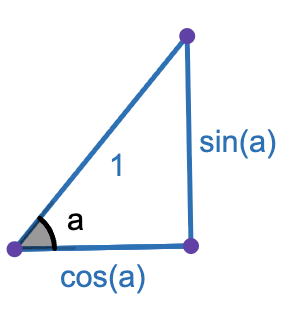
\includegraphics[scale=0.25]{right_triangle}
    \label{fig:Euler_1}
\end{figure}
\end{center}
\end{definition}
もし二つの直角三角形がの直角でない一つの角度が同じ時、二つの三角形は相似となります。なので$\sin(a),\cos(a)$を使うとそれぞれの辺の長さは
\begin{center}
\begin{figure}[h]
	\centering
    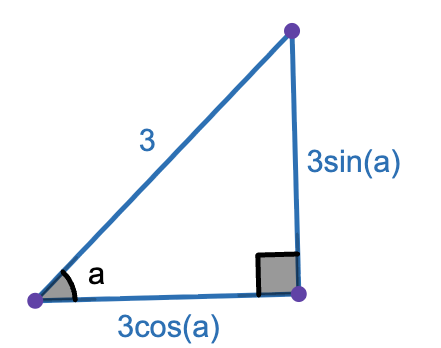
\includegraphics[scale=0.2]{right_triangle_3}
    \label{fig:Euler_1}
\end{figure}
\end{center}
\par\textbf{微分積分：微分の練習}
$(x^n)' = nx^{n-1}$になること、$(f+g)' = f'+g'$（足し算の微分は微分の足し算）と$(af)' = a(f')$(定数との掛け算の微分は微分と定数との掛け算になる）に注意して次の微分を計算してみよう。
\begin{equation*}
3x^2, 5x^4+3x, 6x^5-2x^2
\end{equation*}
\textbf{図形：\ltjruby{正弦定理}{せいげんていり}}
\par \textbf{問題：}次の？に入る数字を$\sin(a),\cos(a),A$をつかって考えてみよう。
\begin{center}
\begin{figure}[h]
	\centering
    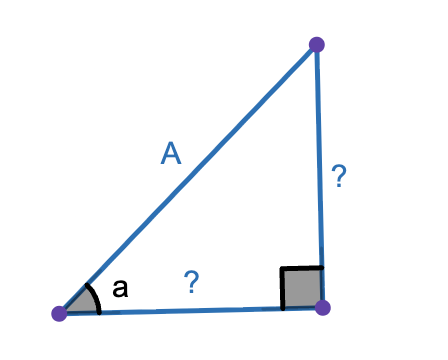
\includegraphics[scale=0.2]{right_triangle_a}
    \label{fig:Euler_1}
\end{figure}
\end{center}

\par \textbf{問題：}つぎの数を計算してみよう。
\begin{equation*}
\sin(60^\circ),\cos(60^\circ),\sin(45^\circ),\cos(45^\circ)
\end{equation*}
下の図を使ってそしてピタゴラスの定理
\begin{equation*}
c^2=a^2+b^2
\end{equation*}
を思い出してみよう。
\begin{center}
\begin{figure}[h]
	\centering
    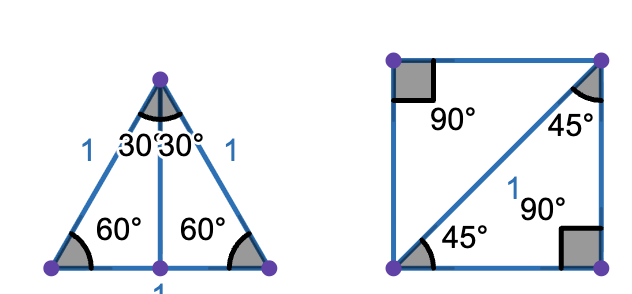
\includegraphics[scale=0.4]{typical_triangles}
    \label{fig:Euler_1}
\end{figure}
\end{center}

\par\textbf{問題：}円周角の定理を思い出そう。
\begin{center}
\begin{figure}[h]
	\centering
    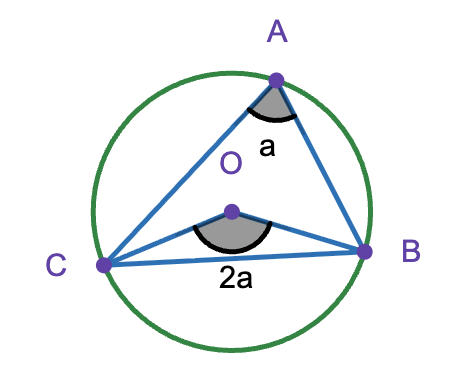
\includegraphics[scale=0.25]{circular_angle}
    \label{fig:Euler_1}
\end{figure}
\end{center}
ここで、ある三角形の外心を考える。
\begin{center}
\begin{figure}[h]
	\centering
    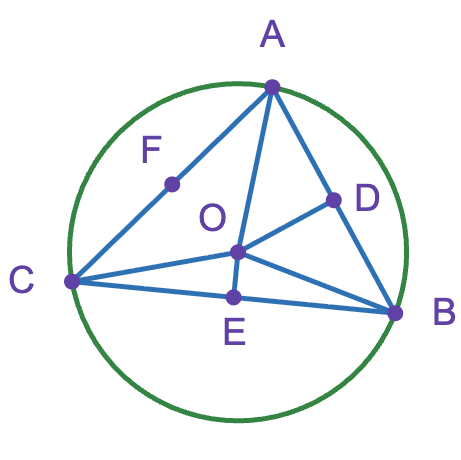
\includegraphics[scale=0.25]{outer_center}
    \label{fig:Euler_1}
\end{figure}
\end{center}
\par\textbf{ステップ１：}円周角の定理を使って$\angle COB$の大きさを$\angle CAB$を使って表してみよう。
\par\textbf{ステップ２：}円周角の定理を使って$\angle COE$の大きさを$\angle COB$の大きさを使って表してみよう。そしてさらにそれを$\angle CAB$を使って表してみよう。
\par\textbf{ステップ３：}$\angle OEC$は$90^\circ$でした。ここに注目して$CE$の長さを$OC,\sin(\angle COE)$を使って表してみよう。
\par\textbf{ステップ４：}$OC$は円の半径。これを$R$とおく。ここでステップ１〜３を使って
\begin{equation*}
2R = {\frac {BC}{\sin(\angle CAB)}}
\end{equation*}
となることを確かめよう。
\par\textbf{グラフ理論：オイラーグラフ}
次のグラフを考えてみる
\begin{center}
\begin{figure}[h]
	\centering
    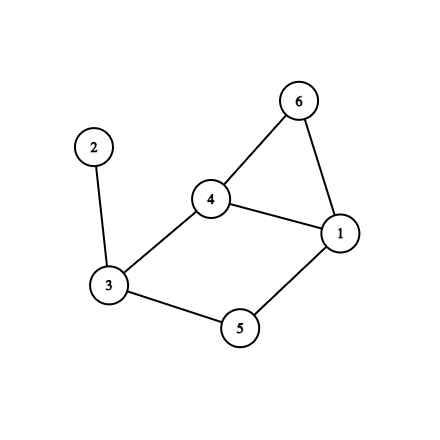
\includegraphics[scale=0.25]{connected_graph_5_16}
    \label{fig:Euler_1}
\end{figure}
\end{center}
辺をいくつか取り除くと次のようなグラフになります
\begin{center}
\begin{figure}[h]
	\centering
    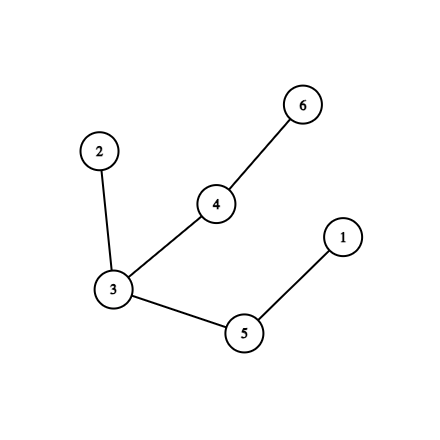
\includegraphics[scale=0.25]{tree_graph_5_16}
    \label{fig:Euler_1}
\end{figure}
\end{center}
このような形のグラフを木グラフと言います。このグラフはいくつかの便利な性質を持ちます。
\begin{center}
\begin{figure}[h]
	\centering
    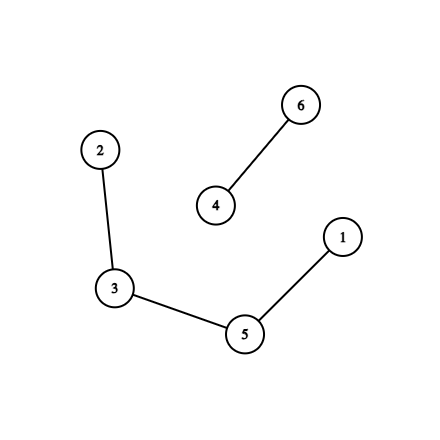
\includegraphics[scale=0.25]{disconnected_graph_5_16}
    \label{fig:Euler_1}
    \caption{どの辺を消してもバラバラになる}
\end{figure}
\end{center}
\begin{center}
\begin{figure}[h]
	\centering
    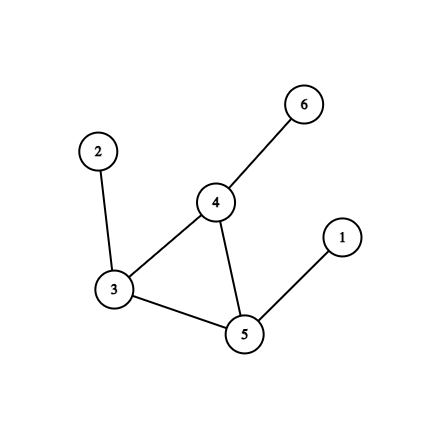
\includegraphics[scale=0.25]{acyclic_graph_5_16}
    \label{fig:Euler_1}
    \caption{どこに辺を足してもサイクルができる（$3,4,5$のサイクルができた）}
\end{figure}
\end{center}
\begin{center}
\begin{figure}[h]
	\centering
    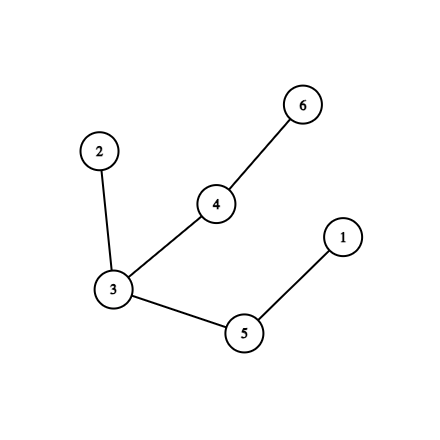
\includegraphics[scale=0.2]{tree_graph_5_16}
    \label{fig:Euler_1}
    \caption{必ず次数が$1$となる頂点がある(頂点$2,6,1$を見てみよう)。このような頂点を\ltjruby{葉}{は}といいます。}
\end{figure}
\end{center}
これらを使って次のことを考えてみよう。
\par\textbf{問題：}一番最初のグラフのように、つながった一つのグラフのことを\ltjruby{連結}{れんけつ}グラフと言います。頂点の次数が全て偶数の連結グラフなら中にサイクルを見つけることができることを証明してみましょう。
\par\textbf{ステップ１：}もし頂点の次数が全て偶数なら連結グラフは木グラフではないことを示そう。（葉の次数はいくつだったかな）
\par\textbf{ステップ２：}連結グラフはいくつかの辺を消すことで木グラフになります。もし頂点の次数が全て偶数なら木グラフを作る時に消さなければいけなかった辺があることを示そう。
\par\textbf{ステップ３：}もし頂点の次数が全て偶数なら連結グラフのなかからサイクルが見つけられることを示そう。（木グラフにする時に消した辺を元に戻すとどうなるかな）
\par\textbf{整数：合同式の逆元}
\begin{equation*}
2\times 3 \equiv 6 \equiv 1\mod{5}
\end{equation*}
のように掛け合わせるとあまりが$1$になる数のペアを次の中から見つけてみよう。(自分自身とのペアも大丈夫、例えば$1\times 1 \equiv 1\mod{5}$。そのようなペアがない数もあるので見つけられない場合は、見つけられなかった数も書いてみよう。（全部やらなくても大丈夫です、できたら$5,6$はやってくれると嬉しいです）。
\begin{enumerate}[i).]
\item $5$で割ったあまりを考えた場合の$1,2,3,4$
\item $7$で割ったあまりを考えた場合の$1,2,3,4,5,6$
\item $6$で割ったあまりを考えた場合の$1,2,3,4,5$
\item $8$で割ったあまりを考えた場合の$1,2,3,4,5,6,7$
\end{enumerate}
\end{document}